\documentclass[noauthor,nooutcomes,12pt,handout]{ximera}

\graphicspath{  
{./}
{./whoAreYou/}
{./drawingWithTheTurtle/}
{./bisectionMethod/}
{./circles/}
{./anglesAndRightTriangles/}
{./lawOfSines/}
{./lawOfCosines/}
{./plotter/}
{./staircases/}
{./pitch/}
{./qualityControl/}
{./symmetry/}
{./nGonBlock/}
}


%% page layout
\usepackage[cm,headings]{fullpage}
\raggedright
\setlength\headheight{13.6pt}


%% fonts
\usepackage{euler}

\usepackage{FiraMono}
\renewcommand\familydefault{\ttdefault} 
\usepackage[defaultmathsizes]{mathastext}
\usepackage[htt]{hyphenat}

\usepackage[T1]{fontenc}
\usepackage[scaled=1]{FiraSans}

%\usepackage{wedn}
\usepackage{pbsi} %% Answer font


\usepackage{cancel} %% strike through in pitch/pitch.tex


%% \usepackage{ulem} %% 
%% \renewcommand{\ULthickness}{2pt}% changes underline thickness

\tikzset{>=stealth}

\usepackage{adjustbox}

\setcounter{titlenumber}{-1}

%% journal style
\makeatletter
\newcommand\journalstyle{%
  \def\activitystyle{activity-chapter}
  \def\maketitle{%
    \addtocounter{titlenumber}{1}%
                {\flushleft\small\sffamily\bfseries\@pretitle\par\vspace{-1.5em}}%
                {\flushleft\LARGE\sffamily\bfseries\thetitlenumber\hspace{1em}\@title \par }%
                {\vskip .6em\noindent\textit\theabstract\setcounter{question}{0}\setcounter{sectiontitlenumber}{0}}%
                    \par\vspace{2em}
                    \phantomsection\addcontentsline{toc}{section}{\thetitlenumber\hspace{1em}\textbf{\@title}}%
                     }}
\makeatother



%% thm like environments
\let\question\relax
\let\endquestion\relax

\newtheoremstyle{QuestionStyle}{\topsep}{\topsep}%%% space between body and thm
		{}                      %%% Thm body font
		{}                              %%% Indent amount (empty = no indent)
		{\bfseries}            %%% Thm head font
		{)}                              %%% Punctuation after thm head
		{ }                           %%% Space after thm head
		{\thmnumber{#2}\thmnote{ \bfseries(#3)}}%%% Thm head spec
\theoremstyle{QuestionStyle}
\newtheorem{question}{}



\let\freeResponse\relax
\let\endfreeResponse\relax

%% \newtheoremstyle{ResponseStyle}{\topsep}{\topsep}%%% space between body and thm
%% 		{\wedn\bfseries}                      %%% Thm body font
%% 		{}                              %%% Indent amount (empty = no indent)
%% 		{\wedn\bfseries}            %%% Thm head font
%% 		{}                              %%% Punctuation after thm head
%% 		{3ex}                           %%% Space after thm head
%% 		{\underline{\underline{\thmname{#1}}}}%%% Thm head spec
%% \theoremstyle{ResponseStyle}

\usepackage[tikz]{mdframed}
\mdfdefinestyle{ResponseStyle}{leftmargin=1cm,linecolor=black,roundcorner=5pt,
, font=\bsifamily,}%font=\wedn\bfseries\upshape,}


\ifhandout
\NewEnviron{freeResponse}{}
\else
%\newtheorem{freeResponse}{Response:}
\newenvironment{freeResponse}{\begin{mdframed}[style=ResponseStyle]}{\end{mdframed}}
\fi



%% attempting to automate outcomes.

%% \newwrite\outcomefile
%%   \immediate\openout\outcomefile=\jobname.oc
%% \renewcommand{\outcome}[1]{\edef\theoutcomes{\theoutcomes #1~}%
%% \immediate\write\outcomefile{\unexpanded{\outcome}{#1}}}

%% \newcommand{\outcomelist}{\begin{itemize}\theoutcomes\end{itemize}}

%% \NewEnviron{listOutcomes}{\small\sffamily
%% After answering the following questions, students should be able to:
%% \begin{itemize}
%% \BODY
%% \end{itemize}
%% }
\usepackage[tikz]{mdframed}
\mdfdefinestyle{OutcomeStyle}{leftmargin=2cm,rightmargin=2cm,linecolor=black,roundcorner=5pt,
, font=\small\sffamily,}%font=\wedn\bfseries\upshape,}
\newenvironment{listOutcomes}{\begin{mdframed}[style=OutcomeStyle]After answering the following questions, students should be able to:\begin{itemize}}{\end{itemize}\end{mdframed}}



%% my commands

\newcommand{\snap}{{\bfseries\itshape\textsf{Snap!}}}
\newcommand{\flavor}{\link[\snap]{https://snap.berkeley.edu/}}
\newcommand{\mooculus}{\textsf{\textbf{MOOC}\textnormal{\textsf{ULUS}}}}


\usepackage{tkz-euclide}
\tikzstyle geometryDiagrams=[rounded corners=.5pt,ultra thick,color=black]
\colorlet{penColor}{black} % Color of a curve in a plot



\ifhandout\newcommand{\mynewpage}{\newpage}\else\newcommand{\mynewpage}{}\fi


\title{Staircases}
\author{Bart Snapp}

\begin{document}
\begin{abstract}
  We use \snap\ to solve the staircase problem.
\end{abstract}
\maketitle

\begin{listOutcomes}
\item{Understand the geometric issues with designing a staircase.}
\item{Interpret solutions for the geometric issues of designing a staircase.}
\item{Reason through how to solve the geometric issues of designing a staircase.}
\item{Critique and dismantle reasonable hypotheses in regard to geometry and arithmetic.}
\end{listOutcomes}



Most building codes have specific restrictions on how a staircase
can be designed. We'll say that a staircase with $n$ stairs looks like this
\begin{center}
  \begin{tikzpicture}[scale = .3]
    \draw[thick]
    (10,0) -- (9,0) -- (9,1) -- (8,1) --
    ( 8,2) -- (7,2) -- (7,3) -- (6,3) --
    ( 6,4) -- (5,4) -- (5,5) -- (4,5) --
    ( 4,6) -- (3,6) -- (3,7) -- (2,7) --
    ( 2,8) -- (1,8) -- (1,9) -- (0,9) --
    (0,10) -- (0,0) -- (10,0);
    \draw [decorate,decoration={brace,amplitude=10pt,mirror},xshift=-4pt,yshift=0pt,]
    (0,10) -- (0,0) node [black,midway,xshift=-1cm] 
          {\footnotesize $n=10$};
    \draw [decorate,decoration={brace,amplitude=10pt},xshift=0pt,yshift=-4pt,]
    (10,0) -- (0,0) node [black,midway,yshift=-.8cm] 
          {\footnotesize $n=10$};     
\end{tikzpicture}
\end{center}
in the case where $n=10$. For safety and comfort, the typical
restrictions on stairs are:
\begin{itemize}
\item The stair-step height can be at most $7\frac{3}{4}''$. 
\item The stair-step depth must be at least $10''$.
\item From step-to-step, these dimensions cannot change (in real-life there is
an allowed variance for these dimensions).
\end{itemize}

So suppose you want to install a staircase in a space that is $15$
feet wide and you need to connect to a floor $10$ feet above the
ground. In this case you must have \emph{at least}
\[
\frac{10}{\left(31/48\right)} \ \text{stairs}
\]
and can have \emph{at most}
\[
\frac{15}{\left(5/6\right)} \ \text{stairs}.
\]


Of course, you must have a \emph{whole} number of stairs. We have two special functions that help out, \emph{floor} and \emph{ceiling}:
\begin{description}
\item[\emph{floor}:] Denoted $\lfloor x\rfloor$, this function, \emph{rounds-down}.
\item[\emph{ceiling}:] Denoted $\lceil x\rceil$ this function, \emph{rounds-up}.
\end{description}
So we see
\[
\text{min number of stairs} = \left\lceil \frac{10}{\left(31/48\right)} \right\rceil
\]
and
\[
\text{max number of stairs} = \left\lfloor \frac{15}{\left(5/6\right)} \right\rfloor.
\]
Both \emph{floor} and \emph{ceiling} are common computer-science
commands and are included in \snap\ via:
\begin{center}
  
\includegraphics{floor-script.png}
  \qquad
  and
  \qquad

\includegraphics{ceiling-script.png}
\end{center}
We'll now use \snap\ to solve the staircase problem.

\mynewpage


\begin{question}
Someone wrote the following \snap\ script to ``solve'' the staircase
problem:

\begin{center}
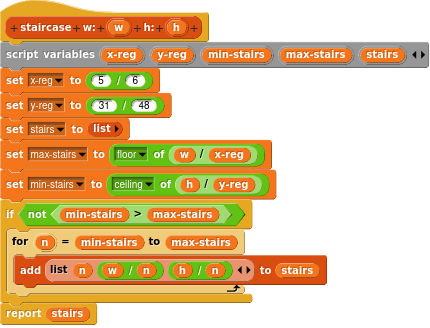
\includegraphics{staircase-script.png}
\end{center}

Run this script in \snap\ for the following values of $w$ and $h$:
\[
w=15\text{ and } h=10, \qquad w=15\text{ and } h=11, \qquad w=15\text{ and } h=13.
\]

Use the values above to help you explain the INPUTS and the OUTPUT of
this code as you would like to have them explained to you. Use words,
pictures, and so on, as needed/helpful in your explanation.
\begin{freeResponse}
  This script has two inputs,
  \begin{align*}
  w &= \text{width of where staircase is needed}\\
  h &= \text{height of where staircase is needed}.
  \end{align*}
  The output is a list of staircase dimensions that meet city
  code.

  When $w=15$ and $h=10$:
  \begin{center}
    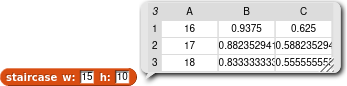
\includegraphics{answer-15-10-script.png}
  \end{center}
  This means we can make three different staircases:
  \begin{enumerate}
  \item $16$ steps, with width $0.938$ feet, and height of $0.625$ feet.
  \item $17$ steps, with width $0.883$ feet, and height of $0.588$ feet.
  \item $18$ steps, with width $0.833$ feet, and height of $0.556$ feet.
  \end{enumerate}

  When $w=15$ and $h=11$:
   \begin{center}
    
\includegraphics{answer-15-11-script.png}
   \end{center}
   This means we can make only one staircase:
   \begin{enumerate}
   \item $18$ steps, with width $0.833$ feet, and height of $0.611$ feet.
   \end{enumerate}


   When $w=15$ and $h=11$:
   \begin{center}
    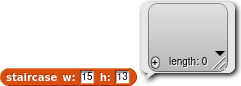
\includegraphics{answer-15-13-script.png}
  \end{center}
   This means we cannot make any staircases that are up to city code in this space.
\end{freeResponse}
\end{question}
\mynewpage

\begin{question}
  Consider again the staircase \snap\ script from the problem above.
  
  EXPLAIN how the script works, block-by-block as you would like to
  have it explained to you. Use words, pictures, and so on, as
  needed/helpful in your explanation.

  \begin{freeResponse}
    \begin{enumerate}
    \item We input the available width $w$ and height $h$.
    \item Next we introduce variables for the horizontal regulation
      $x-reg$, the vertical regulation $y-reg$, the minimum possible
      number of steps $min-stairs$, the maximum number of steps
      $max-stairs$, and finally $stairs$ will be our list of
      solutions.
    \item We set values for $x-reg$, $y-reg$, make $stairs$ a list,
      and get values for $max-stairs$ and $min-stairs$.
    \item\label{stairgoto} Finally, we make sure a staircase is possible by seeing if
      \[
      max-stairs \ge min-stairs
      \]
    \item If one is, we add $min-stairs$ to our list.
    \item We now add $1$ to the minimum number of stairs, and goto step \ref{stairgoto}.
    \end{enumerate}
  \end{freeResponse}
\end{question}
\mynewpage




\begin{question}
  Someone once said,
  \begin{quote}
    The staircase problem isn't hard, you can build a staircase that
    will fit in a space of $w\times h$, if and only if
    \[
    \frac{w}{h} \ge 1.29.
    \]
  \end{quote}
  \begin{enumerate}
    \item How did this person come up with this ``rule-of-thumb?''
    \item Is this correct?
    \item Can you build a staircase where $w=130$ $h=100$? 
  \end{enumerate}
  In each case, explain your reasoning with words, pictures, examples, and so on.
  \begin{freeResponse}
    \begin{enumerate}
    \item This person took minimum depth of $5/6'$ and divided it by
      the maximum height of $31/48'$ to get $1.29$. They then reason that if
      \[
      \frac{w}{h} <1.29.
      \]
      then a stair case CANNOT be built, because the stairs will be
      too narrow and tall. Moreover, they assert that if
      \[
      \frac{w}{h} \ge 1.29.
      \]
    \item They are not correct! For example you cannot build a
      staircase when $w=13'$ and $h=10'$. Behold:
      \begin{center}
        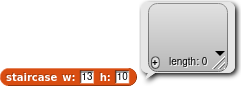
\includegraphics{answer-13-10-result.png}
      \end{center}

    \item You CAN make a staircase that will fit when $w=130'$ and
      $h=100'$. Behold:
      \begin{center}
        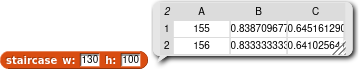
\includegraphics{answer-130-100-result.png}
      \end{center}
      Very interesting!
    \end{enumerate}
  \end{freeResponse}
\end{question}


\end{document}
